% Drawing 138/07-6 -- folder 138, batch 07, archive page 126 (PDF page 127).
% Transcription: un pentagone finement triangulé autour d'un sommet central, les sommets $0$ et $1$ marqués au bord.
% Kind: finely triangulated pentagon. Method 2 (schematic redraw from the facsimile). Status: partial.
% Notes: A pentagon finely triangulated around a central vertex, the vertices 0 and 1 marked on the boundary. The fan is redrawn with rays to the vertices and to two points on each side, plus a ring of chords; the exact number of triangles cannot be counted on the page (overinked), so it is not encoded.
% Coordinates: 1 unit = 1 mm = 1/100 of the crop width (bbox in page fractions: [0.685, 0.179, 0.836, 0.286]).
% Redrawn by Claude (claude-opus-5-5), issue #73, 2026-11-07; not checked by a human; not compiled (no TeX in the session).
% Rights: reproduces part of the work -- behind RENDER_TRANSCRIPTS, never published by itself.
\documentclass[tikz,border=3pt]{standalone}
\usepackage{amsmath,amssymb}
\usetikzlibrary{patterns,arrows.meta}
\tikzset{pencil/.style={black!45}, struck/.style={black!35}, mark/.style={circle,draw,inner sep=1.3pt}, pt/.style={circle,fill,inner sep=0.9pt}, opt/.style={circle,draw,fill=white,inner sep=1.1pt}}
\begin{document}
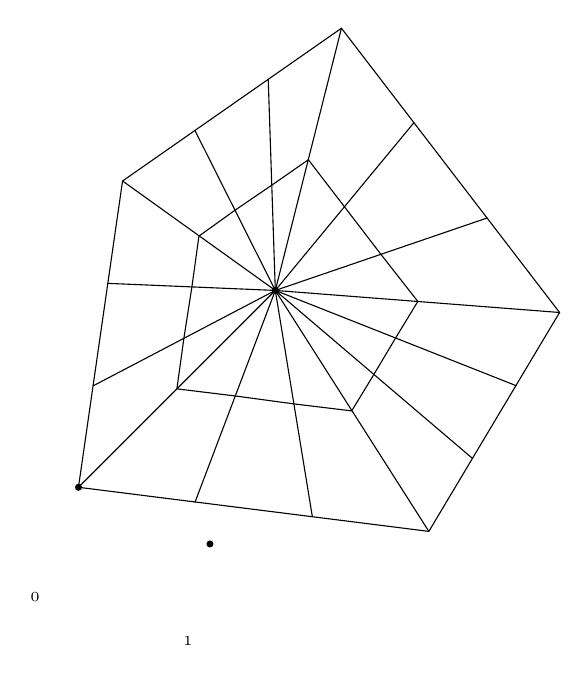
\begin{tikzpicture}[x=1mm,y=1mm,line cap=round,line join=round,font=\scriptsize]
\draw (27.8,-33.3) -- (55.6,-13.9) -- (83.3,-50) -- (66.7,-77.8) -- (22.2,-72.2) -- cycle;
\draw (47.2,-47.2) -- (27.8,-33.3);
\draw (47.2,-47.2) -- (37,-26.9);
\draw (47.2,-47.2) -- (46.3,-20.4);
\draw (47.2,-47.2) -- (55.6,-13.9);
\draw (47.2,-47.2) -- (64.8,-25.9);
\draw (47.2,-47.2) -- (74.1,-38);
\draw (47.2,-47.2) -- (83.3,-50);
\draw (47.2,-47.2) -- (77.8,-59.3);
\draw (47.2,-47.2) -- (72.2,-68.5);
\draw (47.2,-47.2) -- (66.7,-77.8);
\draw (47.2,-47.2) -- (51.9,-75.9);
\draw (47.2,-47.2) -- (37,-74.1);
\draw (47.2,-47.2) -- (22.2,-72.2);
\draw (47.2,-47.2) -- (24.1,-59.3);
\draw (47.2,-47.2) -- (25.9,-46.3);
\draw (37.5,-40.3) -- (42.1,-37) -- (46.8,-33.8) -- (51.4,-30.6) -- (56,-36.6) -- (60.6,-42.6) -- (65.3,-48.6) -- (62.5,-53.2) -- (59.7,-57.9) -- (56.9,-62.5) -- (49.5,-61.6) -- (42.1,-60.6) -- (34.7,-59.7) -- (35.6,-53.2) -- (36.6,-46.8) -- cycle;
\node[pt] at (47.2,-47.2) {};
\node[pt] at (22.2,-72.2) {};
\node[pt] at (38.9,-79.4) {};
\node[inner sep=1pt] at (16.7,-86.1) {\tiny $0$};
\node[inner sep=1pt] at (36.1,-91.7) {\tiny $1$};
\end{tikzpicture}
\end{document}
